
本研究における可視化システムは,
Atlassian社が提供するタスク管理サービスTrello\cite{trello}と連携して動作する.
Trelloは,タスクの情報をカード,
タスクの状態をボードとして管理するサービスである.
利用者は,タスクを実行した際に,
カードを次のボードに移動させる.
これにより,プロジェクトメンバ間でタスクの進捗状況を共有することができる.
また,Trelloでは,カードに複数人の作業担当者を設定することが可能である.
そこで,本システムでは,
同じカードに割り振られた作業担当者は,
協働でタスクを行ったという前提で,
Trello上でのカードの移動履歴を利用することで,
プロジェクトメンバが協働で作業を行っている様子を可視化した.

% 従来の概念図と,本システムによる可視化の比較
% MEMO: N個のベン図は表現可能
% https://nunuki.hatenablog.com/entry/2017/12/31/175302
従来までの実践共同体とメンバの関係性は,
図\ref{cop}と図\ref{overlap}で示したように,
実践共同体とメンバを,
領域と要素のように表現されてきた.
% しかし,実践共同体とプロジェクトメンバの関係性を可視化する際に,
% 図\ref{cop}の様な表現を採用することを考えると,
% 実践共同体の中心と,メンバの距離を表すことはできるが,
% メンバ間の距離や,
% メンバ間のなす角が余計な情報として表されてしまう.
% もし,距離やなす角によって,
% 協働でタスクを行った回数などを表すとしても,
% メンバが四人以上のプロジェクトを対象とした場合に,
% 二次元平面で全てのメンバの関係性を表現することはできない.
しかし,実践共同体とプロジェクトメンバの関係性を可視化する際に,
図\ref{cop}の様な表現を採用することを考えると,
参加深度と同時に,
メンバ同士の関係性を距離によって表現することは困難だと考えられる.
また,布置を可視化する際に,
図\ref{overlap}の様な表現を採用することを考えた場合にも,
3つ以上の実践共同体を表現しようとした際に,
閉曲線が複雑化してしまう可能性が考えられる.
そこで,本研究では,
プロジェクトメンバをノード,
プロジェクトメンバが協働でタスクを行った履歴をエッジとすることで,
プロジェクトの状況をネットワーク構造によって表現した.
これにより,複雑なメンバの関係性や,
異なる実践共同体間の関係性を観察することを可能にした.
本システムによって可視化したプロジェクトメンバの関係性を,
図\ref{cop-map-graph}に示す.

\begin{figure}[h]
  \centering
  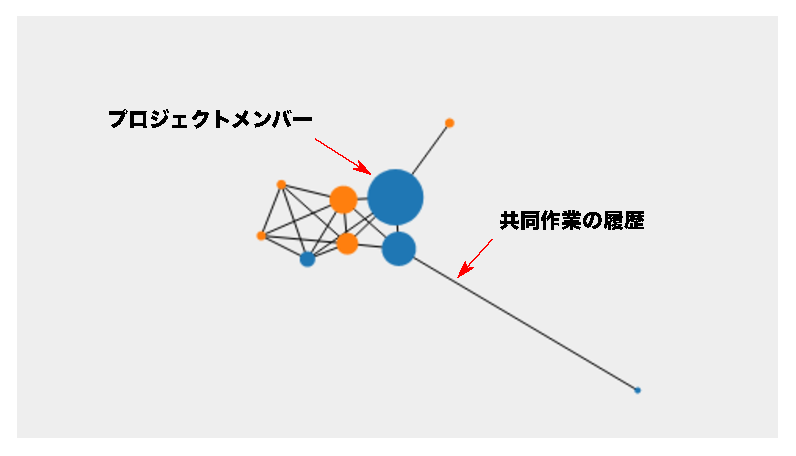
\includegraphics[width=0.5\textwidth]{img/cop-map-graph.eps}
  \caption{本システムによってプロジェクトメンバの関係性を可視化した様子}
  \label{cop-map-graph}
\end{figure}

本システムでは,ノードのレイアウト手法として,力学モデルを採用している.
また,協働でタスクを行った回数によってエッジの強度を変化させることで,
多くのタスクを協働で行うほど,
ノード間の距離は近くなるように配置される.
これにより,頻繁に協働でタスクを行っているプロジェクトメンバを確認することができる.
また,そのプロジェクトメンバが異なる実践共同体に所属していた場合に,
異なる実践共同体の間で,協働的にタスクが行われているかを観察することができる.
本システムによって可視化された,
協働で行われたタスクの様子を図\ref{cop-map-task}に示す.

\begin{figure}[h]
  \centering
  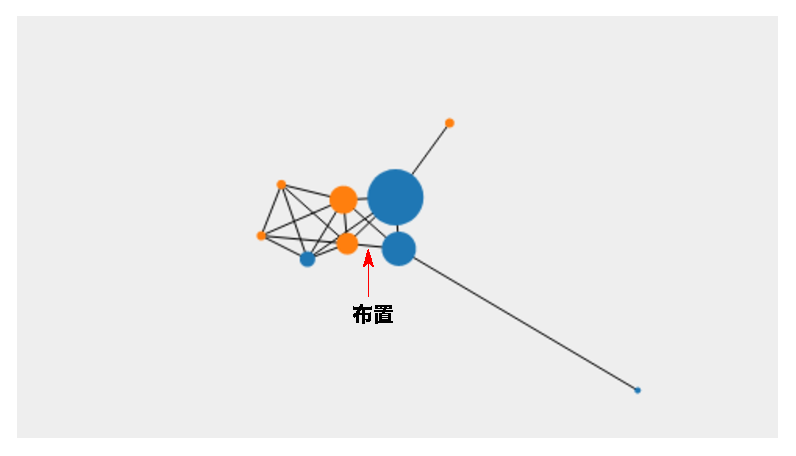
\includegraphics[width=0.5\textwidth]{img/cop-map-task.eps}
  \caption{本システムによって可視化された協働で行われたタスク}
  \label{cop-map-task}
\end{figure}

また,プロジェクトメンバの所属先によってノードの色を変化させることで,
異なる実践共同体に所属するプロジェクトメンバが,
協働でタスクを行っている様子を観察することを可能にしている.
これにより,異なる色のノードがエッジでつながっている様子から,
布置を観察することができる.
本システムによって観察される布置の例を,
図 \ref{cop-map-overlap}に示す.

\begin{figure}[h]
  \centering
  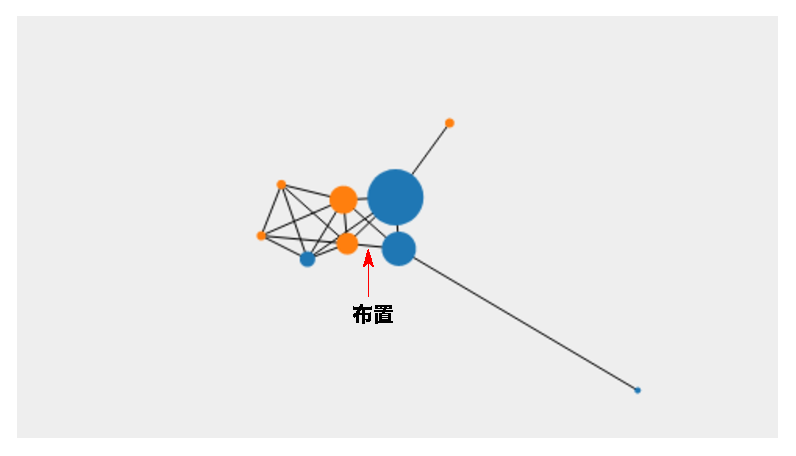
\includegraphics[width=0.5\textwidth]{img/cop-map-overlap.eps}
  \caption{本システムによって可視化された布置}
  \label{cop-map-overlap}
\end{figure}

さらに,タスクを行った回数の合計値によってノードの大きさを変化させている.
これにより,プロジェクトメンバが正統的周辺参加である可能性を観察することが可能である.
その一例として,ノードは小さいが,他のノードとの繋がりが見られる場合が挙げられる.
この場合は,観察対象となるプロジェクトメンバは,
タスクを行った回数は少ないが,
リソースへのアクセスが可能な状態だと考える事ができる.
本システムによって,
観察される正統的周辺参加である可能性のあるプロジェクトメンバを図\ref{cop-map-lpp}に示す.

\begin{figure}[h]
  \centering
  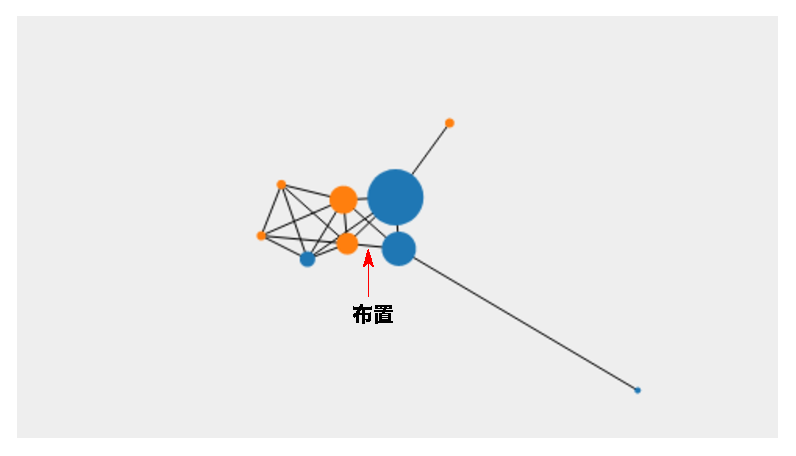
\includegraphics[width=0.5\textwidth]{img/cop-map-lpp.eps}
  \caption{本システムによって観察される正統的周辺参加である可能性のあるプロジェクトメンバ}
  \label{cop-map-lpp}
\end{figure}

以上のネットワーク構造を,プロジェクトの時系列順に変化させることで,
プロジェクトメンバの関係性の変化を観察することを可能にしている.
これにより,ノードの軌跡から,
進行状況によって変化していく,
プロジェクトメンバの軌跡を観察することを可能にしている.
本システムによって観察されるプロジェクトメンバの軌跡を,
図\ref{cop-map-trajectory}に示す.

\begin{figure}[h]
  \centering
  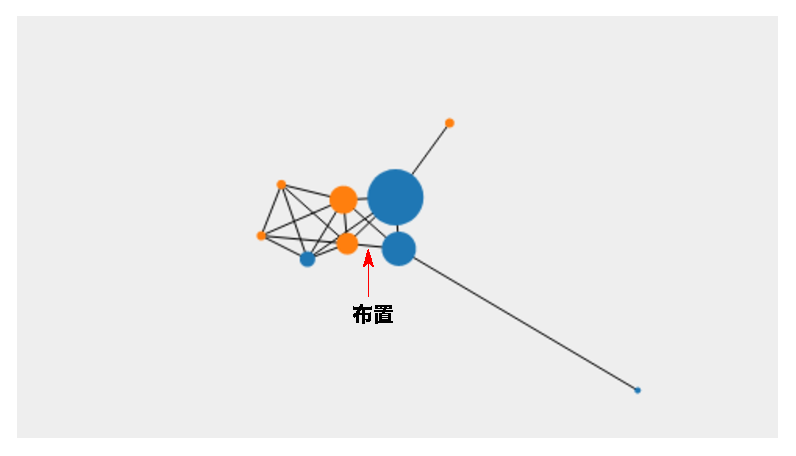
\includegraphics[width=0.5\textwidth]{img/cop-map-trajectory.eps}
  \caption{本システムによって観察されるプロジェクトメンバの軌跡}
  \label{cop-map-trajectory}
\end{figure}

また,本システムではインタラクティブにデータを観察することが可能である.
本システムで可能なインタラクションは,
ノードのドラッグアンドドロップと,ノードへのマウスオーバーである.
ノードをドラッグアンドドロップすることによって,
ネットワークのレイアウトを調整することが可能である.
また,メンバの詳細情報を確認する際には,
ノードにマウスオーバーすることで,
そのノードに対応するユーザ名を確認することが可能である.
これらのインタラクションにより,
より詳細にプロジェクトメンバの関係性を観察することが可能である.
インタラクションによって詳細情報を表示している様子を,
図\ref{cop-map-detail}に示す.

\begin{figure}[h]
  \centering
  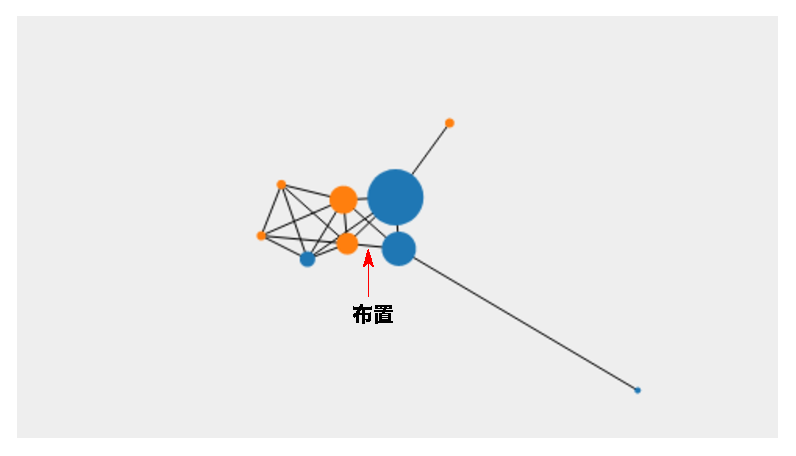
\includegraphics[width=0.5\textwidth]{img/cop-map-detail.eps}
  \caption{インタラクションによって詳細情報を表示している様子}
  \label{cop-map-detail}
\end{figure}
